\documentclass{article}
\usepackage{tikz}
\usepackage{pgfplots}

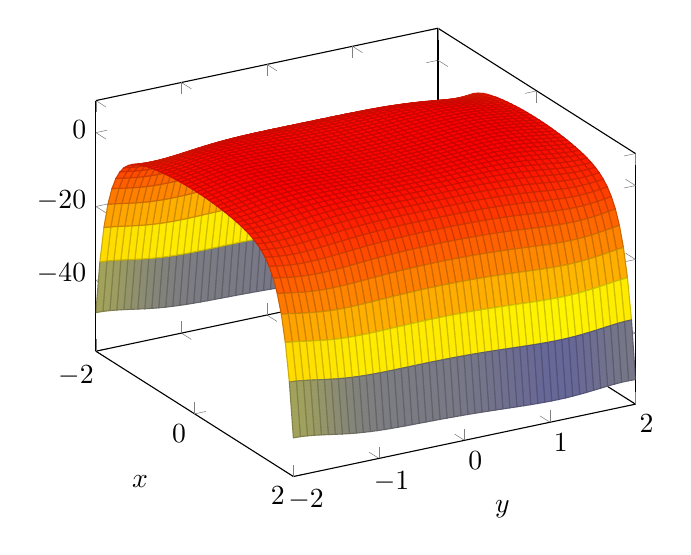
\begin{tikzpicture}
\begin{axis}[
xlabel=$x$,
ylabel=$y$,
domain=-2:2,
y domain=-2:2,
colormap/viridis,
view={60}{30}
]
\addplot3[surf, colormap/hot, samples=50] {sin(deg(x^2+y^2)) - exp(x^2+sin(y)) + 3};
\end{axis}
\end{tikzpicture}
\section{3D Integral 2}
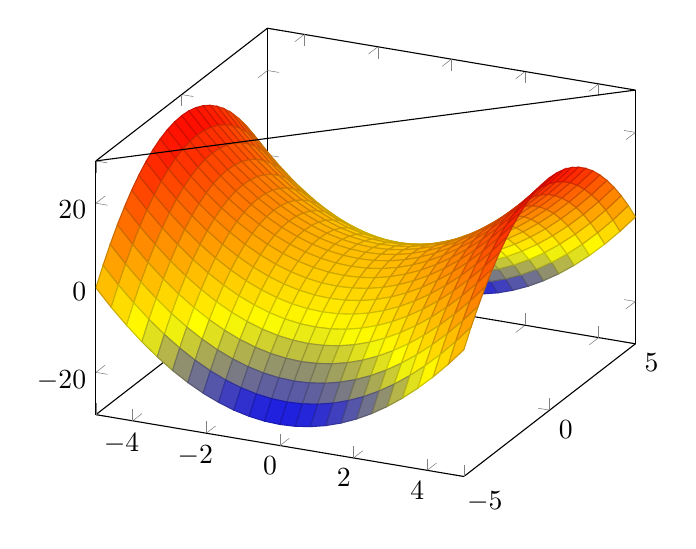
\begin{tikzpicture}
\begin{axis}
\addplot3[surf] {x^2 - y^2};
\draw (rel axis cs:0,0,1) -- (rel axis cs:1,1,1);
\end{axis}
\end{tikzpicture}
